\documentclass[border=8pt]{standalone}
\usepackage[utf8]{inputenc}
\usepackage[T1]{fontenc}
\usepackage[scaled]{helvet}
\renewcommand{\familydefault}{\sfdefault}
\usepackage{tikz}
\usetikzlibrary{shapes.multipart,positioning,arrows.meta}
\tikzset{
  cls/.style={rectangle split, rectangle split parts=3, draw, thick, fill=white,
    rectangle split part fill={black!8,white,white}, align=left, font=\scriptsize,
    inner sep=3pt, text width=#1},
  cls/.default=3.6cm,
  assoc/.style={thick},
  dep/.style={thick, dashed, -{Stealth[length=2mm]}},
  mult/.style={font=\scriptsize, fill=white, inner sep=1pt}
}
\newcommand{\cname}[1]{\centering\textbf{#1}}
\begin{document}
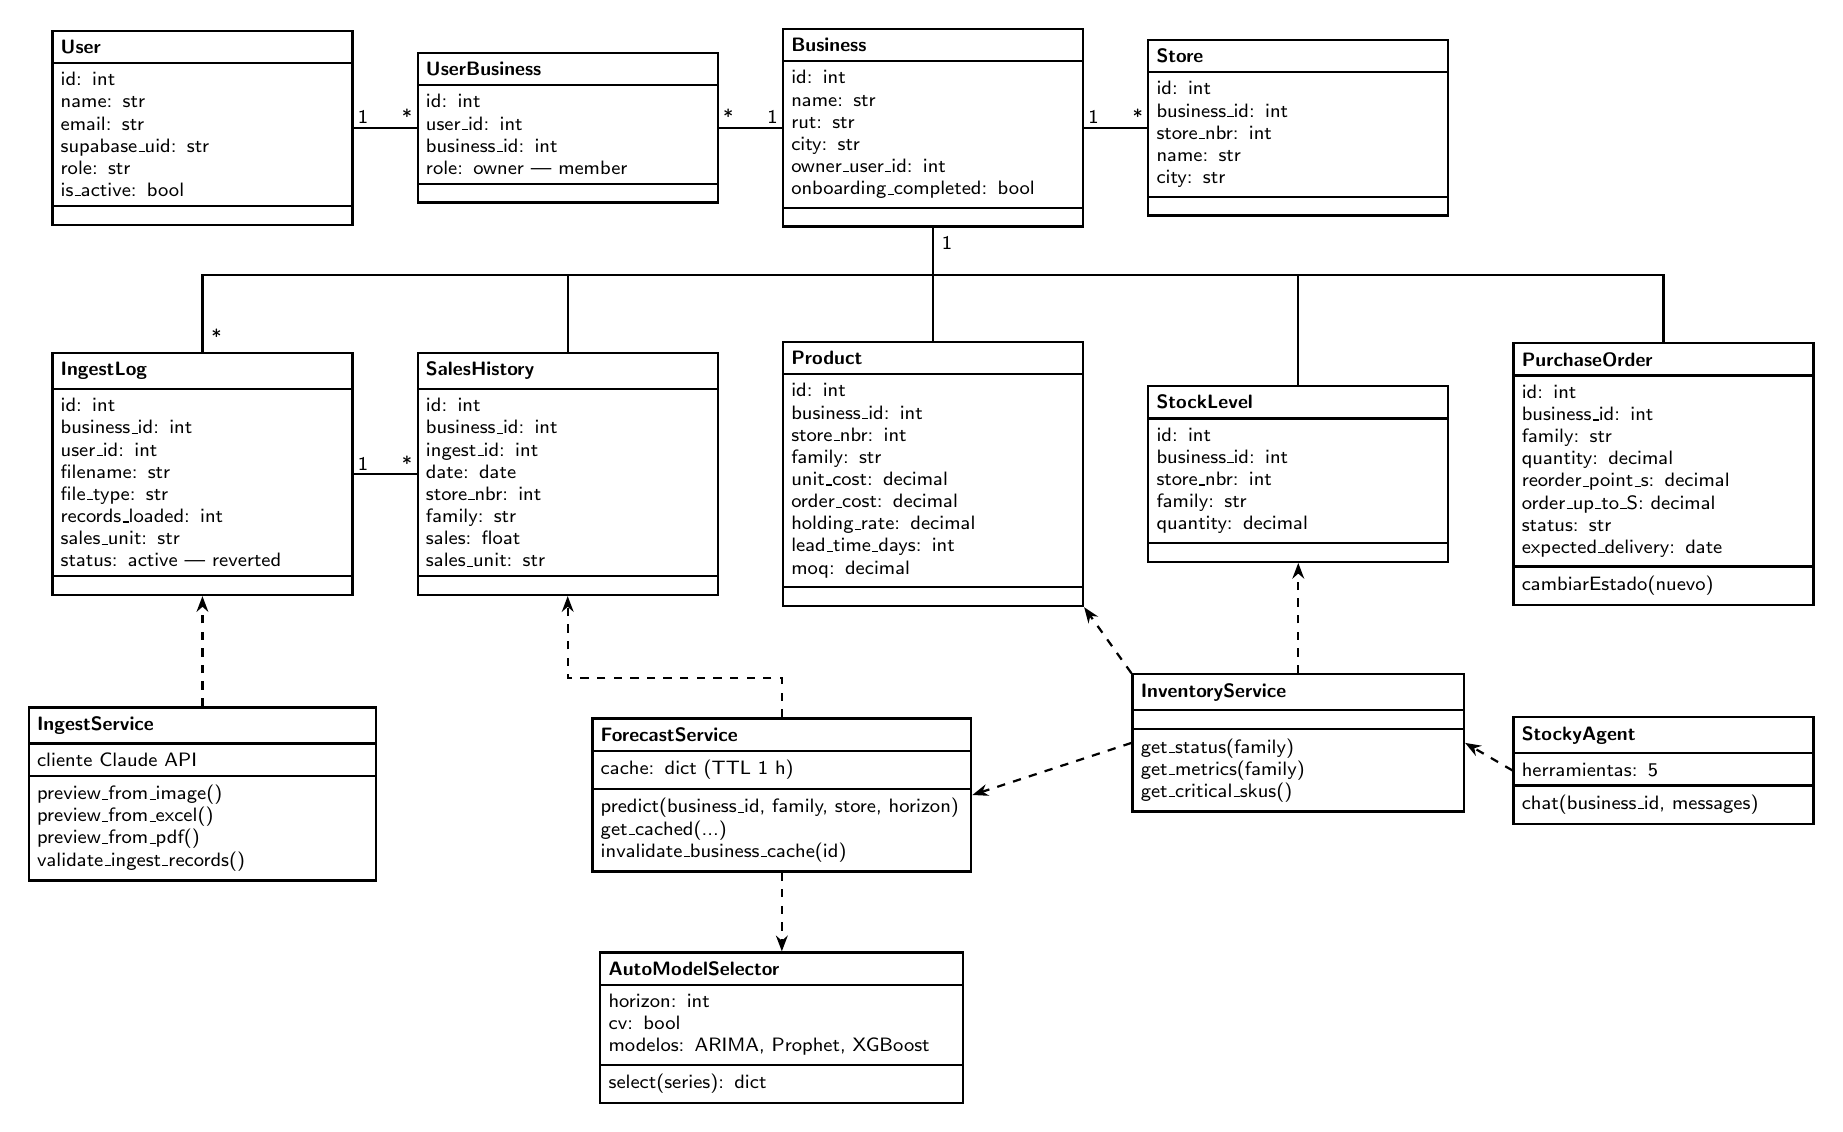
\begin{tikzpicture}[node distance=1.0cm and 0.8cm]
% Fila 1
\node[cls] (user) {\cname{User}
 \nodepart{second} id: int\\ name: str\\ email: str\\ supabase\_uid: str\\ role: str\\ is\_active: bool
 \nodepart{third} };
\node[cls, right=of user] (ub) {\cname{UserBusiness}
 \nodepart{second} id: int\\ user\_id: int\\ business\_id: int\\ role: owner | member
 \nodepart{third} };
\node[cls, right=of ub] (biz) {\cname{Business}
 \nodepart{second} id: int\\ name: str\\ rut: str\\ city: str\\ owner\_user\_id: int\\ onboarding\_completed: bool
 \nodepart{third} };
\node[cls, right=of biz] (store) {\cname{Store}
 \nodepart{second} id: int\\ business\_id: int\\ store\_nbr: int\\ name: str\\ city: str
 \nodepart{third} };
% Fila 2
\node[cls, below=1.6cm of user] (log) {\cname{IngestLog}
 \nodepart{second} id: int\\ business\_id: int\\ user\_id: int\\ filename: str\\ file\_type: str\\ records\_loaded: int\\ sales\_unit: str\\ status: active | reverted
 \nodepart{third} };
\node[cls, right=of log] (sales) {\cname{SalesHistory}
 \nodepart{second} id: int\\ business\_id: int\\ ingest\_id: int\\ date: date\\ store\_nbr: int\\ family: str\\ sales: float\\ sales\_unit: str
 \nodepart{third} };
\node[cls, right=of sales] (prod) {\cname{Product}
 \nodepart{second} id: int\\ business\_id: int\\ store\_nbr: int\\ family: str\\ unit\_cost: decimal\\ order\_cost: decimal\\ holding\_rate: decimal\\ lead\_time\_days: int\\ moq: decimal
 \nodepart{third} };
\node[cls, right=of prod] (stock) {\cname{StockLevel}
 \nodepart{second} id: int\\ business\_id: int\\ store\_nbr: int\\ family: str\\ quantity: decimal
 \nodepart{third} };
\node[cls, right=of stock] (po) {\cname{PurchaseOrder}
 \nodepart{second} id: int\\ business\_id: int\\ family: str\\ quantity: decimal\\ reorder\_point\_s: decimal\\ order\_up\_to\_S: decimal\\ status: str\\ expected\_delivery: date
 \nodepart{third} cambiarEstado(nuevo)};
% Fila 3: servicios
\node[cls=4.2cm, below=1.4cm of log.south, anchor=north] (ing) {\cname{IngestService}
 \nodepart{second} cliente Claude API
 \nodepart{third} preview\_from\_image()\\ preview\_from\_excel()\\ preview\_from\_pdf()\\ validate\_ingest\_records()};
\node[cls=4.6cm, below=1.4cm of prod.south west, anchor=north] (fs) {\cname{ForecastService}
 \nodepart{second} cache: dict (TTL 1 h)
 \nodepart{third} predict(business\_id, family, store, horizon)\\ get\_cached(...)\\ invalidate\_business\_cache(id)};
\node[cls=4.0cm, below=1.4cm of stock.south, anchor=north] (inv) {\cname{InventoryService}
 \nodepart{second} 
 \nodepart{third} get\_status(family)\\ get\_metrics(family)\\ get\_critical\_skus()};
\node[cls=3.6cm, below=1.4cm of po.south, anchor=north] (stocky) {\cname{StockyAgent}
 \nodepart{second} herramientas: 5
 \nodepart{third} chat(business\_id, messages)};
\node[cls=4.4cm, below=1.0cm of fs] (ams) {\cname{AutoModelSelector}
 \nodepart{second} horizon: int\\ cv: bool\\ modelos: ARIMA, Prophet, XGBoost
 \nodepart{third} select(series): dict};
% Asociaciones
\draw[assoc] (user) -- node[mult, pos=0.15, above]{1} node[mult, pos=0.85, above]{*} (ub);
\draw[assoc] (ub) -- node[mult, pos=0.15, above]{*} node[mult, pos=0.85, above]{1} (biz);
\draw[assoc] (biz) -- node[mult, pos=0.15, above]{1} node[mult, pos=0.85, above]{*} (store);
\draw[assoc] (biz.south) -- ++(0,-0.6) -| (log.north);
\draw[assoc] (biz.south) -- ++(0,-0.6) -| (sales.north);
\draw[assoc] (biz.south) -- ++(0,-0.6) -| (prod.north);
\draw[assoc] (biz.south) -- ++(0,-0.6) -| (stock.north);
\draw[assoc] (biz.south) -- ++(0,-0.6) -| (po.north);
\node[mult, anchor=west] at ([xshift=2pt,yshift=-0.2cm]biz.south) {1};
\node[mult, anchor=west] at ([xshift=2pt,yshift=0.2cm]log.north) {*};
\draw[assoc] (log) -- node[mult, pos=0.15, above]{1} node[mult, pos=0.85, above]{*} (sales);
% Dependencias
\draw[dep] (ing.north) -- (log.south);
\draw[dep] (fs.north) -- ++(0,0.5) -| (sales.south);
\draw[dep] (fs.south) -- (ams.north);
\draw[dep] (inv.north) -- (stock.south);
\draw[dep] (inv.north west) -- (prod.south east);
\draw[dep] (inv.west) -- (fs.east);
\draw[dep] (stocky.west) -- (inv.east);
\end{tikzpicture}
\end{document}
